\documentclass[aspectratio=169]{beamer}
% You can change aspectratio=169 to 43 or 1610 to adjust slide dimensions.

% Theme settings
\usetheme{default}
\usecolortheme{default}

% Basic beamer adjustments
\setbeamertemplate{navigation symbols}{}
\setbeamertemplate{footline}[frame number]

% Packages
\usepackage{graphicx}
\usepackage{amsmath}
\usepackage{booktabs}
\usepackage{multicol} % for optional multi-column layouts
\usepackage{hyperref} % for hyperlinks (if desired)

% Title Info
\title{Mechanics of Materials - Week 12: Thin-Walled Pressure Vessels}
\subtitle{Cylindrical \& Spherical Vessels}
\author{Viggo Hansen}
\date{April 2, 2025}

%------------------------------------------------------
\begin{document}

% Title Slide
\begin{frame}
  \titlepage
\end{frame}

% Optional: Repeated Outline at sub-sections
\AtBeginSection[]
{
  \begin{frame}{Outline}
    \tableofcontents[currentsection]
  \end{frame}
}

% Main Outline Slide
\begin{frame}{Outline}
  \tableofcontents
\end{frame}

%------------------------------------------------------
\section{Introduction to Pressure Vessels}

\begin{frame}{What Are Pressure Vessels?}
  \begin{itemize}
    \item Containers designed to hold gases or liquids under pressure.
    \item Examples include boilers, gas tanks, water pipes, and even aerosol cans.
    \item A \textbf{thin-walled vessel} assumption applies when the wall thickness $t$ is relatively small compared to the inner radius $r$ (rule of thumb: $r/t \geq 10$).
  \end{itemize}
  \vfill
  \begin{figure}
    \centering
    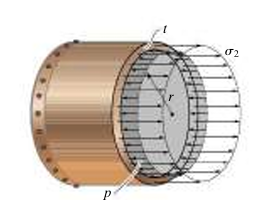
\includegraphics[width=0.25\textwidth]{cyl.png} % Replace with an actual image
    \caption{Schematic of a thin-walled cylindrical vessel}
  \end{figure}
\end{frame}

\begin{frame}{Why Thin-Walled Assumption?}
  \begin{itemize}
    \item Simplifies stress analysis significantly.
    \item Enables closed-form solutions for hoop and longitudinal stresses.
    \item Common in practice for pipes, pressurized hoses, and large storage tanks.
  \end{itemize}
  \note{When $r/t$ is not large enough, more advanced methods (e.g., thick-walled analysis) must be used.}
\end{frame}

%------------------------------------------------------
\section{Cylindrical Pressure Vessels}

\begin{frame}{Stresses in Cylindrical Vessels}
  \begin{itemize}
    \item Internal gauge pressure: $p$.
    \item Two primary normal stresses:
      \begin{itemize}
        \item \textbf{Hoop (circumferential) stress}: $\sigma_{\theta}$ or $\sigma_{\text{hoop}}$.
        \item \textbf{Longitudinal (axial) stress}: $\sigma_{\text{long}}$.
      \end{itemize}
  \end{itemize}
  \vfill
  \begin{block}{Key Equations (Thin-Walled)}
    \[
      \sigma_{\text{hoop}} = \sigma_1 = \frac{p r}{t}, 
      \qquad
      \sigma_{\text{long}} = \sigma_2 = \frac{p r}{2t}.
    \]
  \end{block}
  \note{Notice that $\sigma_{\text{hoop}}$ is twice as large as $\sigma_{\text{long}}$.}
\end{frame}

\begin{frame}{Derivation of Hoop Stress (Brief)}
  \begin{itemize}
    \item Consider a half-cylinder cut by a plane parallel to the axis.
    \item Force due to internal pressure acts on the cross-sectional area (length $\approx 2r$).
    \item Hoop stress acts along the circumference on the “cut” edges.
    \item Equilibrium of horizontal forces leads to:
    \[
      \sigma_{\text{hoop}} \cdot (t \times \text{length}) 
      \;=\; p \cdot (\text{internal area}).
    \]
  \end{itemize}
  \[
    \sigma_{\text{hoop}} = \frac{p r}{t}.
  \]
  \begin{figure}
    \centering
    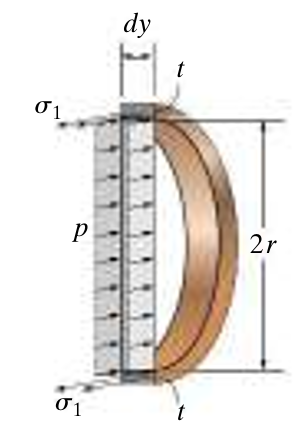
\includegraphics[width=0.2\textwidth]{hoop.png} % Replace with an actual figure
    \caption{Hoop stress free-body diagram}
  \end{figure}
\end{frame}

\begin{frame}{Engineering Considerations}
  \begin{itemize}
    \item \textbf{Factor of Safety (F.S.)}: Typically, use $\sigma_{\text{allowed}} = \frac{\sigma_{\text{yield}}}{\text{F.S.}}$.
    \item \textbf{End Caps}: Axial loads on heads can introduce additional stresses.
    \item \textbf{Material Selection}: Must withstand stresses and possible corrosion, temperature effects.
    \item \textbf{Welding/Joints}: Often the weak link in pressure vessels.
  \end{itemize}
\end{frame}

\begin{frame}{Full 2D Stress Tensor in Cylindrical Vessels}
  \begin{itemize}
    \item Combines hoop and longitudinal stresses into a 2D stress state at a point.
    \item Assume: longitudinal direction ($x$), hoop direction ($y$), no shear ($\tau_{xy} = 0$).
  \end{itemize}
  \vfill
  \begin{block}{Stress Tensor}
    \[
      \sigma = \begin{bmatrix}
        \sigma_{\text{long}} & 0 \\
        0 & \sigma_{\text{hoop}}
      \end{bmatrix}
      = \begin{bmatrix}
        \frac{p r}{2t} & 0 \\
        0 & \frac{p r}{t}
      \end{bmatrix}
    \]
  \end{block}
  \note{This tensor represents the biaxial stress state; radial stress ($\sigma_r$) is negligible for thin walls.}
\end{frame}

%------------------------------------------------------
\section{Spherical Pressure Vessels}

\begin{frame}{Stresses in Spherical Vessels}
  \begin{itemize}
    \item Due to symmetry, stress is uniform in all directions in a sphere.
    \item Magnitude of spherical stress is identical to the \emph{longitudinal} stress in a cylindrical vessel.
  \end{itemize}
  \vfill
  \begin{block}{Key Equation (Thin-Walled Sphere)}
    \[
      \sigma_{\text{sphere}} = \frac{p r}{2t}.
    \]
  \end{block}
  \note{This is half the hoop stress of a comparable cylinder under the same pressure.}
\end{frame}

\begin{frame}{Free-Body Diagram (Spherical)}
  \begin{itemize}
    \item If you “cut” a sphere by a plane, the internal pressure acts over a circular cross section.
    \item The internal tensile stress in the spherical wall resists the force due to pressure.
  \end{itemize}
  \vfill
  \begin{figure}
    \centering
    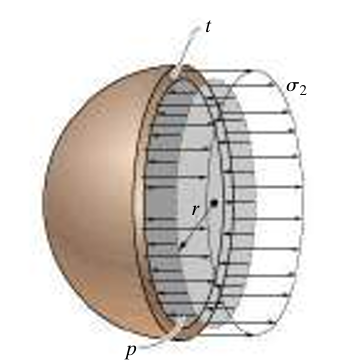
\includegraphics[width=0.2\textwidth]{sphere.png} % Replace with an actual figure
    \caption{Spherical vessel free-body diagram}
  \end{figure}
\end{frame}

%------------------------------------------------------
\section{Summary \& Applications}

\begin{frame}{Key Takeaways}
  \begin{itemize}
    \item \textbf{Thin-Walled Cylinders:}
      \[
        \sigma_{\text{hoop}} = \frac{p r}{t}, 
        \quad
        \sigma_{\text{long}} = \frac{p r}{2t}.
      \]
    \item \textbf{Thin-Walled Spheres:}
      \[
        \sigma_{\text{sphere}} = \frac{p r}{2t}.
      \]
    \item \textbf{When to apply}:
      \begin{itemize}
        \item $r / t \gtrapprox 10$ for the thin-walled assumption.
        \item Uniform internal pressure.
      \end{itemize}
    \item \textbf{Engineering Concern}: Always ensure proper safety factors for material strength, welds, and design codes (ASME, etc.).
  \end{itemize}
\end{frame}

\begin{frame}{Further Reading}
  \begin{itemize}
    \item Mechanics of Materials texts (e.g., Gere, Beer \& Johnston).
    \item ASME Boiler and Pressure Vessel Code (BPVC) for practical design standards.
    \item API standards for piping and petroleum-related vessels.
  \end{itemize}
  \vfill
  \centering
\end{frame}

\end{document}